\chapter{Simulation results}
\label{chap-simulation}

This chapter includes ...

\section{Generating RODD disturbances}

Outline notes:
\begin{itemize}
	\item RODDs are easy to generate.
	\item Describe the three types of RODD disturbance shown in Fig. \ref{fig:rodd-sim-plots}.
\end{itemize}

\begin{figure}[htp]
	\centering
	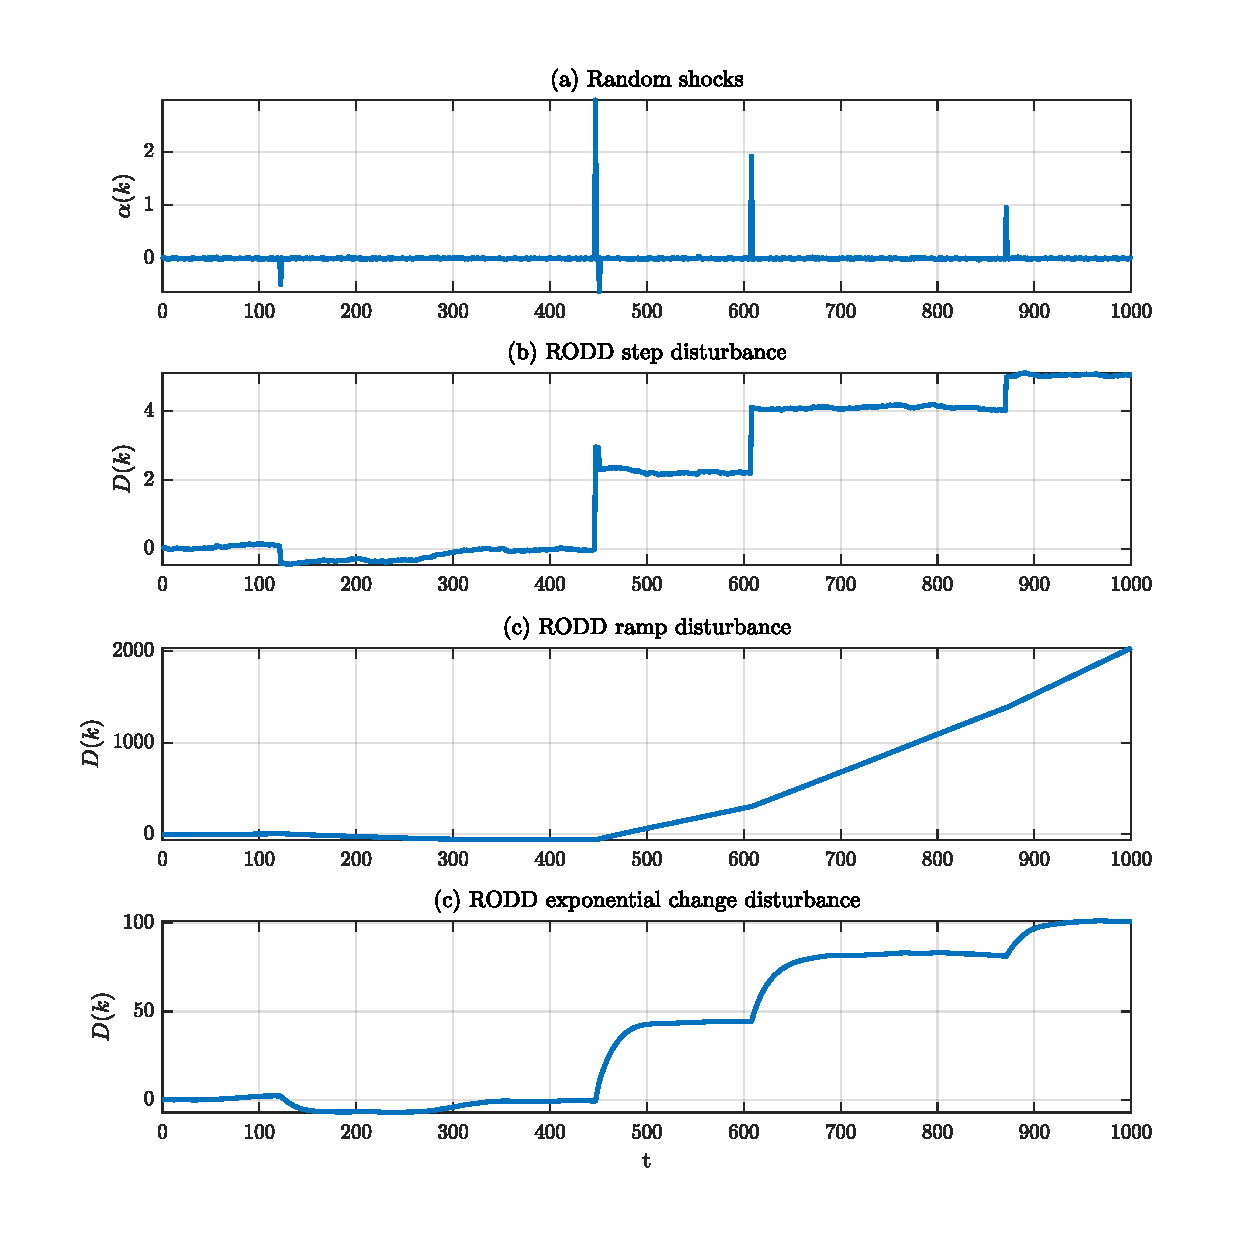
\includegraphics[width=15cm]{images/rodd-sim-plots.pdf}
	\caption{Examples of RODD disturbances}
	\label{fig:rodd-sim-plots}
\end{figure}


\section{Estimating RODD disturbances}

\subsection{SISO linear system}

Outline notes:
\begin{itemize}
	\item Describe linear system with RODD step disturbance at input.
	\item Fig. \ref{fig:sim-sys-diag-siso}: Functional diagram of simulated system.
	\item Define SISO linear process model.
\begin{equation}
	\frac{B(z^{-1})}{A(z^{-1})} = \frac{0.3z^{-1}}{1-0.7z^{-1}}
\end{equation}
\begin{equation}
	\frac{C(z^{-1})}{D(z^{-1})} = \frac{1}{1-z^{-1}}
\end{equation}
\begin{equation}
	\begin{split}
	x_{a}(k+1) & =\left[\begin{array}{cc}
		0.7 & 1 \\
		0 & 1
	\end{array}\right] x_{a}(k)+\left[\begin{array}{l}
		1 \\
		0
	\end{array}\right] u(k)+\left[\begin{array}{l}
		0 \\
		1
	\end{array}\right] w_{p}(k) \\
	y(k) & =\left[\begin{array}{cc}
	0.3 & 0
\end{array}\right] x_{a}(k)
\end{split}
\end{equation}
	\item Figure \ref{fig:rodd-obs-sim-1-4-ioplot}: input-output data from simulated system
	\item Different methods of tuning of single Kalman filters (KF1, KF2, KF3).
	\item Reference the necessary trade-off explained in methods section.
	\item Summary table of Kalman filter parameters
	\item Figure \ref{fig:rod-obs-sim-1-4-est-KF}: Kalman filter simulation results—hidden state and output estimates plot
	\item Figure \ref{fig:rod-obs-sim-1-4_est_err}: Kalman filter simulation results—cumulative output error plot
\end{itemize}

\begin{figure}[htp]
	\centering
	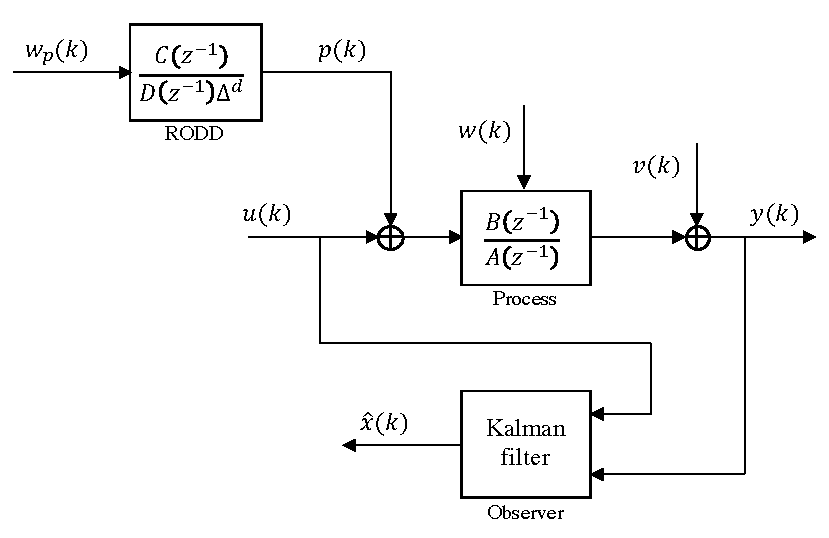
\includegraphics[width=11.5cm]{images/sim-sys-diag-siso.pdf}
	\caption{Functional diagram of the simulated system with observer}
	\label{fig:sim-sys-diag-siso}
\end{figure}

\begin{figure}[htp]
	\centering
	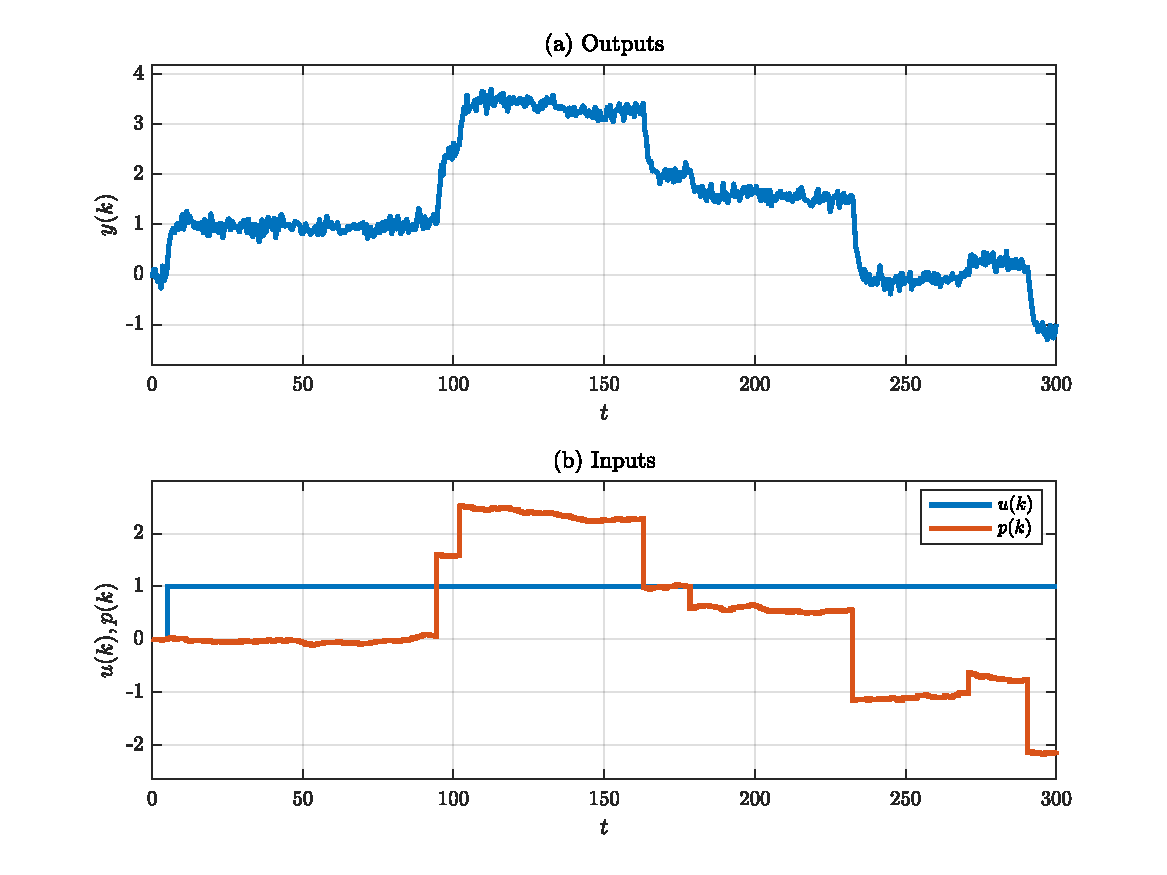
\includegraphics[width=15cm]{images/rod-obs-sim-1-4-ioplot.pdf}
	\caption{Simulation of linear system with a RODD input disturbance}
	\label{fig:rodd-obs-sim-1-4-ioplot}
\end{figure}

\begin{figure}[htp]
	\centering
	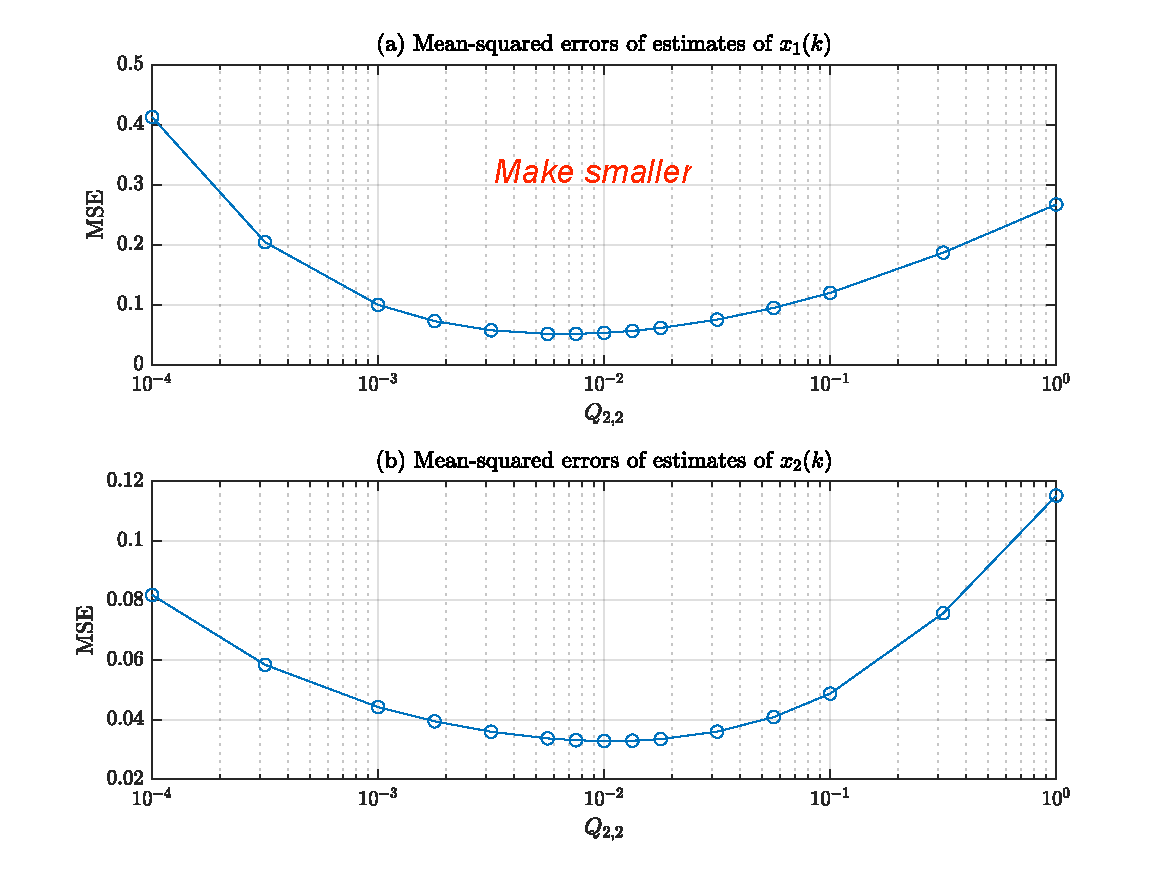
\includegraphics[width=15cm]{images/rod-obs-tuning-KF2-plot-DRAFT.pdf}
	\caption{Tuning of Kalman filter to minimise mean-squared estimation error}
	\label{fig:rod-obs-tuning-KF2-plot}
\end{figure}

\begin{figure}[htp]
	\centering
	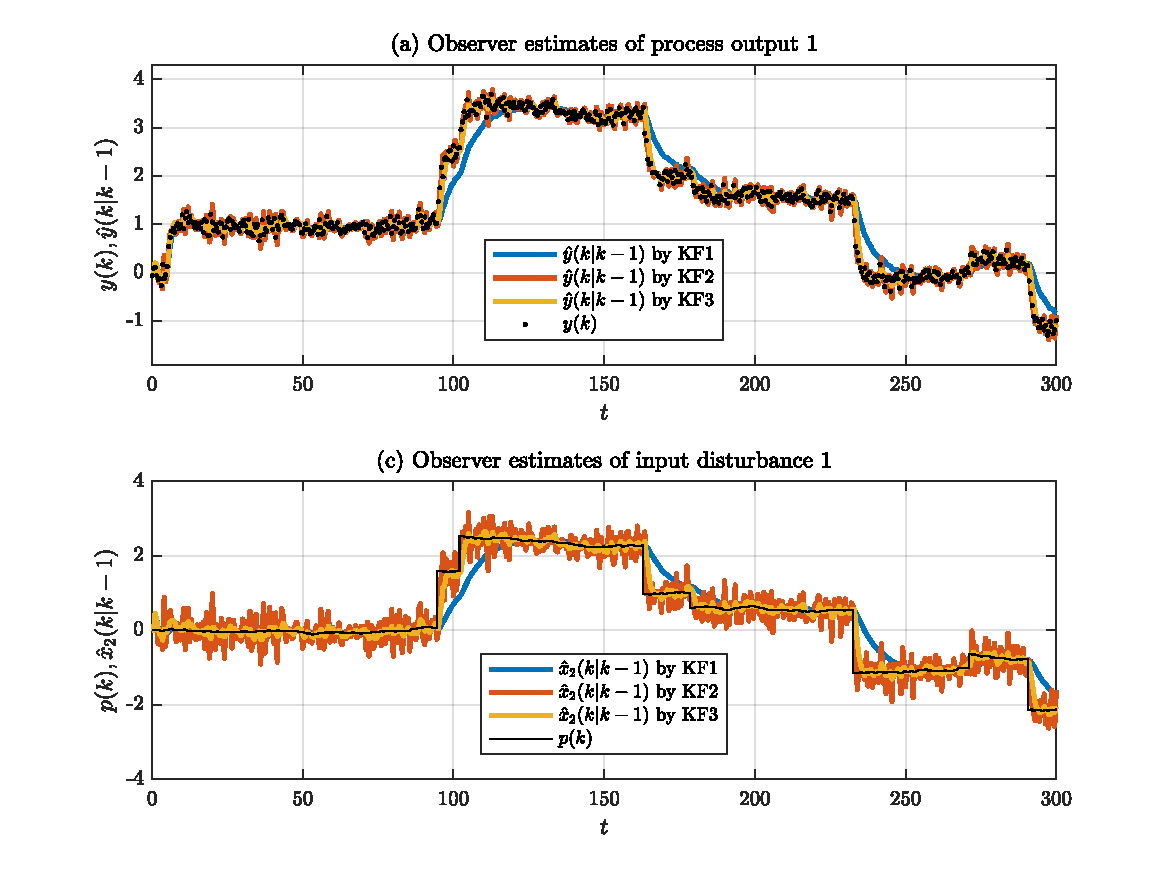
\includegraphics[width=15cm]{images/rod-obs-sim-1-4-est-KF.pdf}
	\caption{Kalman filter estimates}
	\label{fig:rod-obs-sim-1-4-est-KF}
\end{figure}

\begin{figure}[htp]
	\centering
	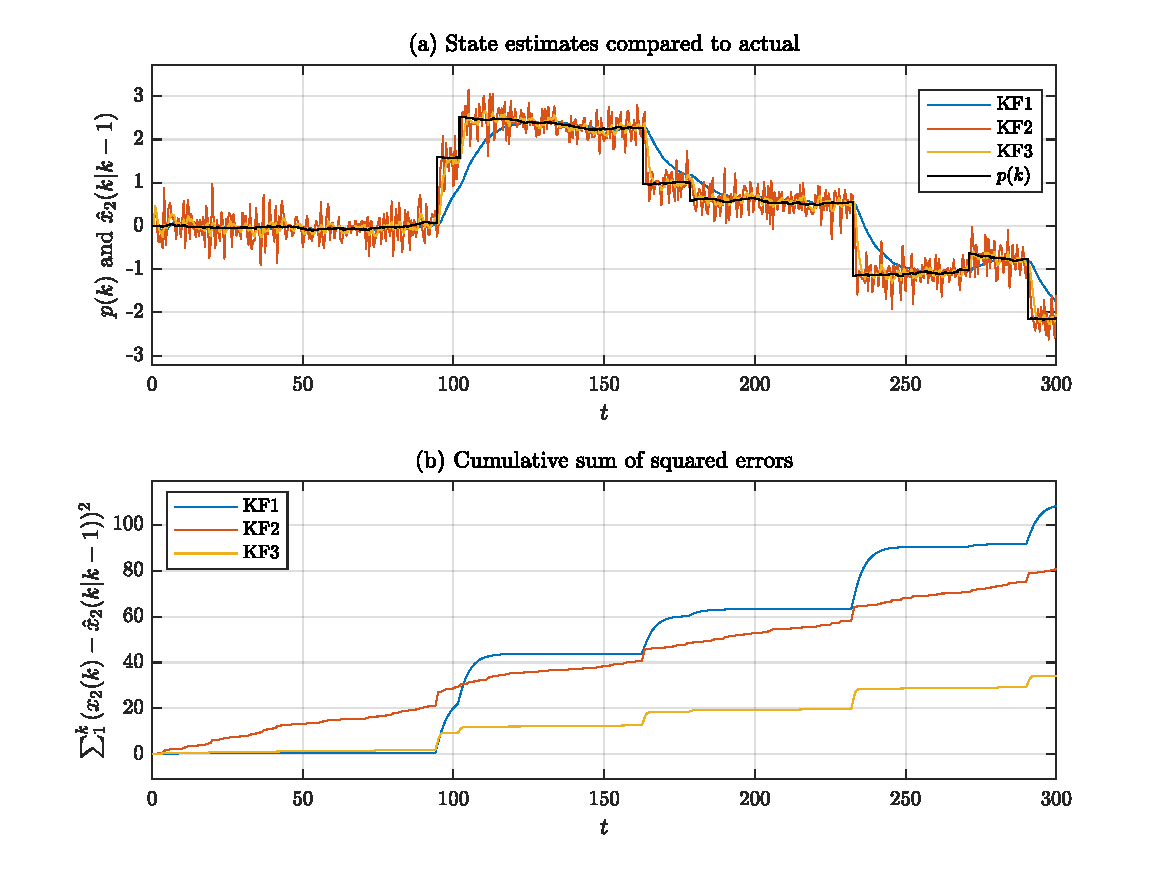
\includegraphics[width=15cm]{images/rod-obs-sim-1-4_est_err.pdf}
	\caption{Kalman filter estimates of input disturbance}
	\label{fig:rod-obs-sim-1-4_est_err}
\end{figure}

\begin{itemize}
	\item Tuning of sequence fusion (Robertson et al.) sub-optimal observer.
	\item Figure showing two sets of sequences considered.
	\item Summary table of parameter optimization results.
	\item Sequence fusion observer simulation results - state and output estimates vs. true values.
	\item Analysis of internal workings to explain apparent problems with responding to shocks.
	\item Waterfall plots of observer internal variables—p(Gamma|Y), K, trace(P).
	\item Tuning of sequence pruning (Eriksson and Isaksson) sub-optimal observer.
	\item Summary table of parameter optimization results.
	\item Sequence pruning observer simulation results - state and output estimates vs. true values.
	\item Summary table of all multi-model observer parameters.
	\item Comparison of multi-model observer simulation results—hidden state and output estimates plot.
	\item Comparison of multi-model observer simulation results—cumulative estimation errors.
	\item Comparison of observer simulation results—MSE bar chart summary.
	\item Summary table comparing performance metrics for all three observers (KF3, MKF-SF, MKF-SP) - metrics: MSE, MSE-transitions, MSE-steady-state, variance-steady-state, MSD-steady-state.
	\item Discussion: Compare and contrast -> sequence pruning approach (Eriksson and Isaksson) works better.
	\item Conclude on pros, cons of each algorithm and decision to use sequence pruning for grinding simulation experiments.
\end{itemize}

\begin{figure}[htp]
	\centering
	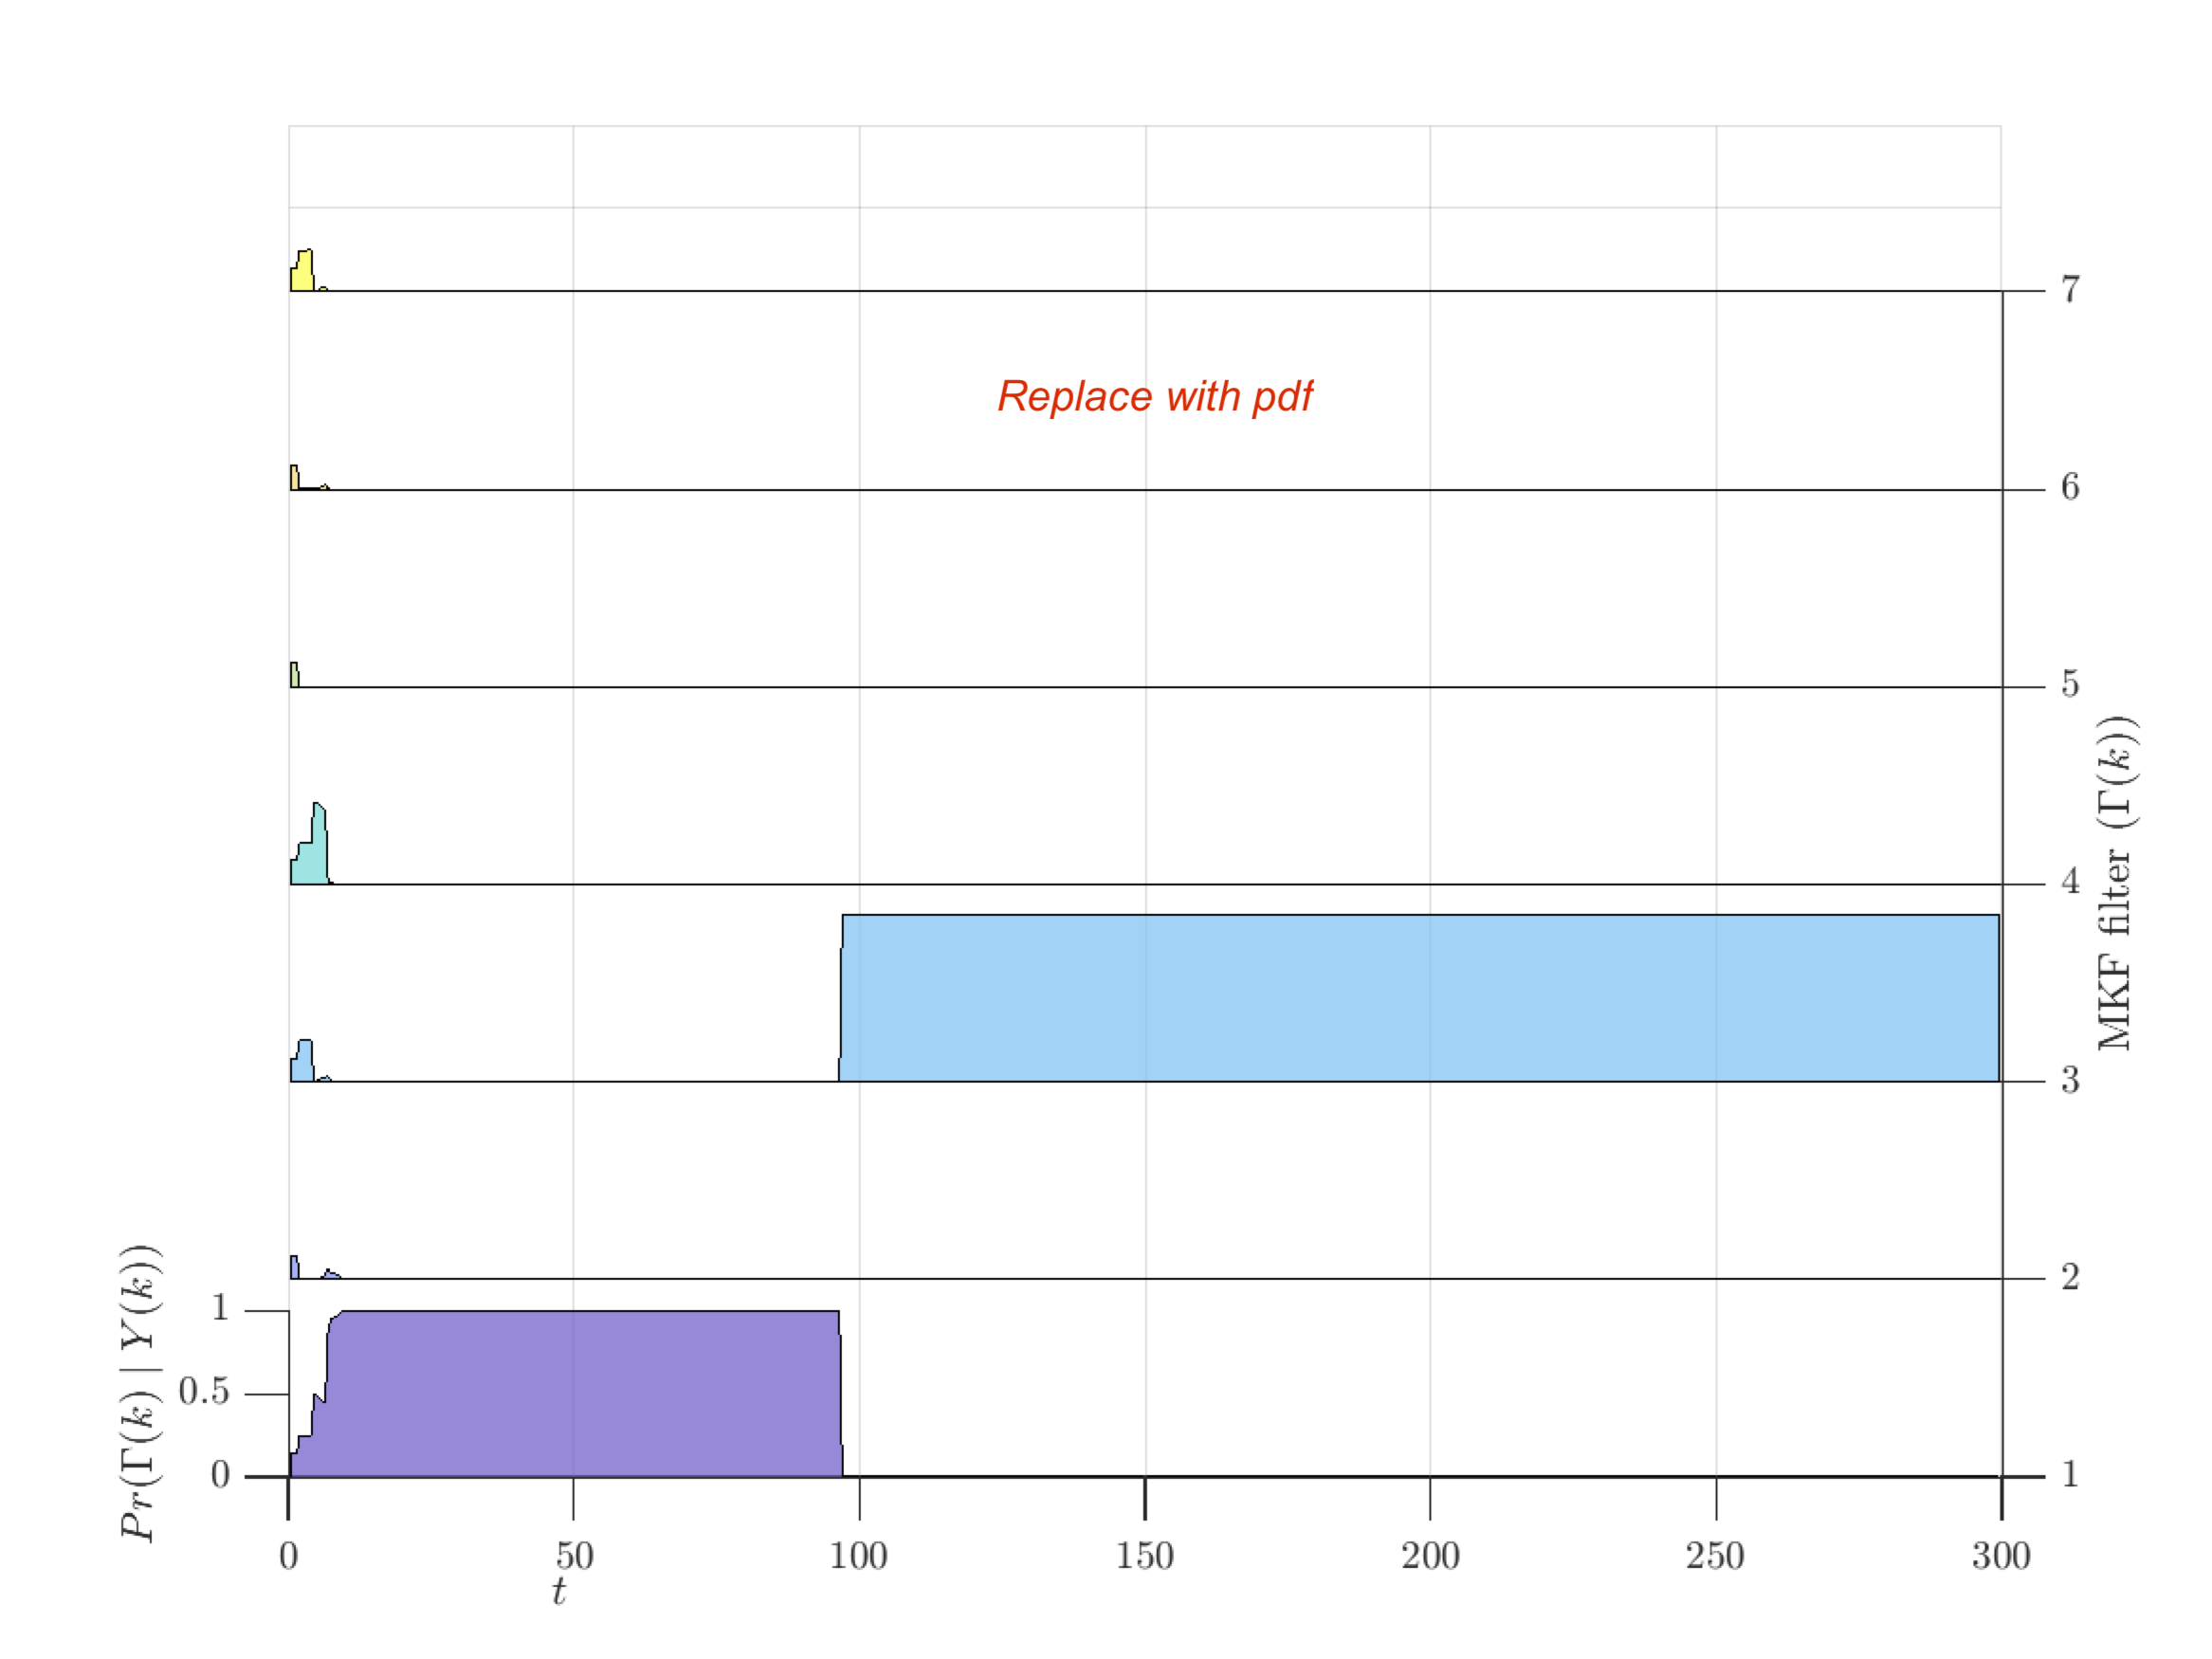
\includegraphics[width=15cm]{images/rod-obs-sim-1-4-wfplot-DRAFT.png}
	\caption{Evolution of conditional probabilities with sequence fusion}
	\label{fig:rod-obs-sim-1-4-wfplot}
\end{figure}

\begin{figure}[htp]
	\centering
	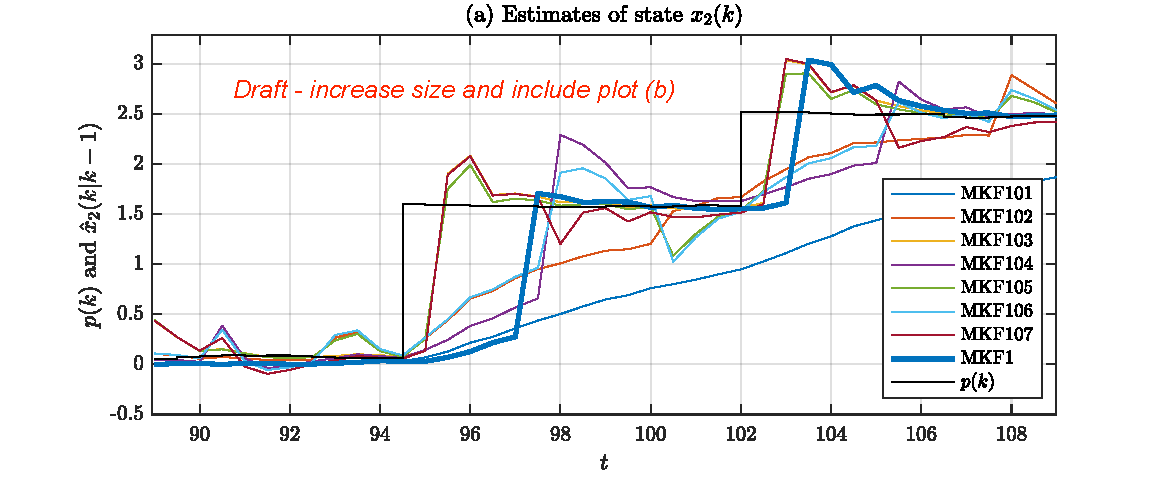
\includegraphics[width=14cm]{images/rod-obs-sim-1-4-est-MKF-SF-plot-DRAFT.pdf}
	\caption{Filter estimates of sequence fusion observer during step disturbances}
	\label{fig:rod-obs-sim-1-4-est-MKF-SF-plot-DRAFT}
\end{figure}

\begin{figure}[htp]
	\centering
	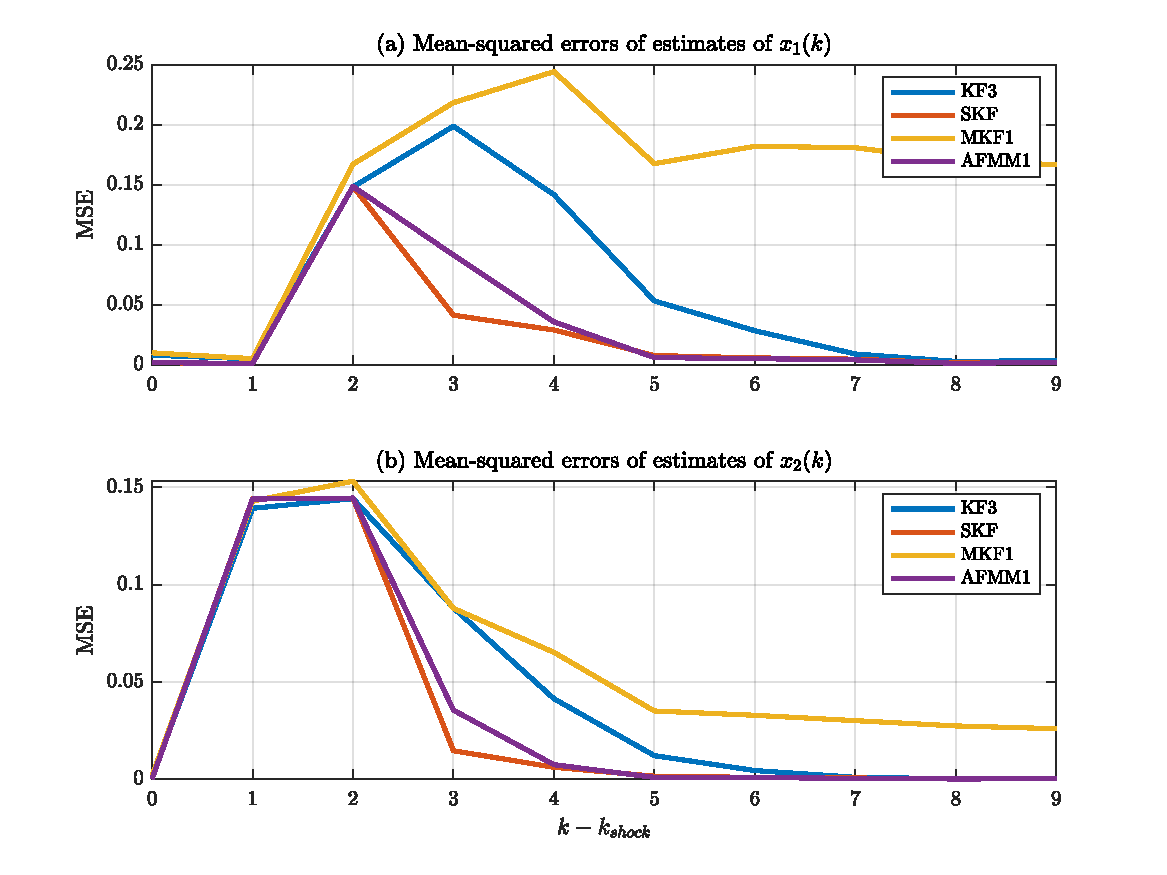
\includegraphics[width=14cm]{images/rod_obs_sim2_7_mse_ashocks.pdf}
	\caption{Average errors of observer estimates after shock disturbances}
	\label{fig:rod_obs_sim2_7_mse_ashocks}
\end{figure}

\begin{figure}[htp]
	\centering
	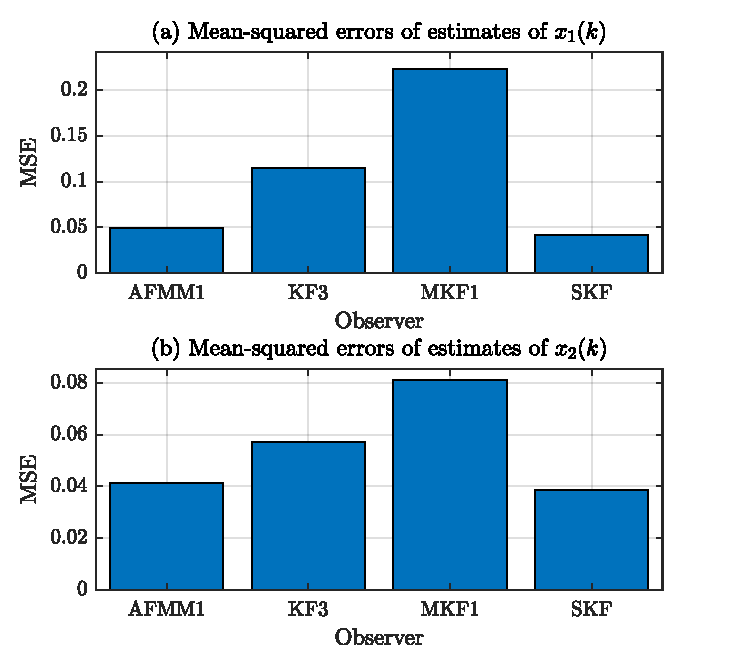
\includegraphics[width=11cm]{images/rod-obs-sim-1-7-MSE-DRAFT.pdf}
	\caption{Comparison of mean-squared errors of observer estimates}
	\label{fig:rod-obs-sim-1-7-MSE}
\end{figure}

\subsection{MIMO linear system OR non-linear system (t.b.d.)}

\begin{itemize}
	\item Include similar results using a MIMO system—either the 2x2 linear system or the 0x2 non-linear system used by Robertson et al. (Aromatization process).
	\item Figure \ref{fig:rodd-obs-sim-2-4-ioplot}: input-output data from simulated system
\end{itemize}

\begin{figure}[htp]
	\centering
	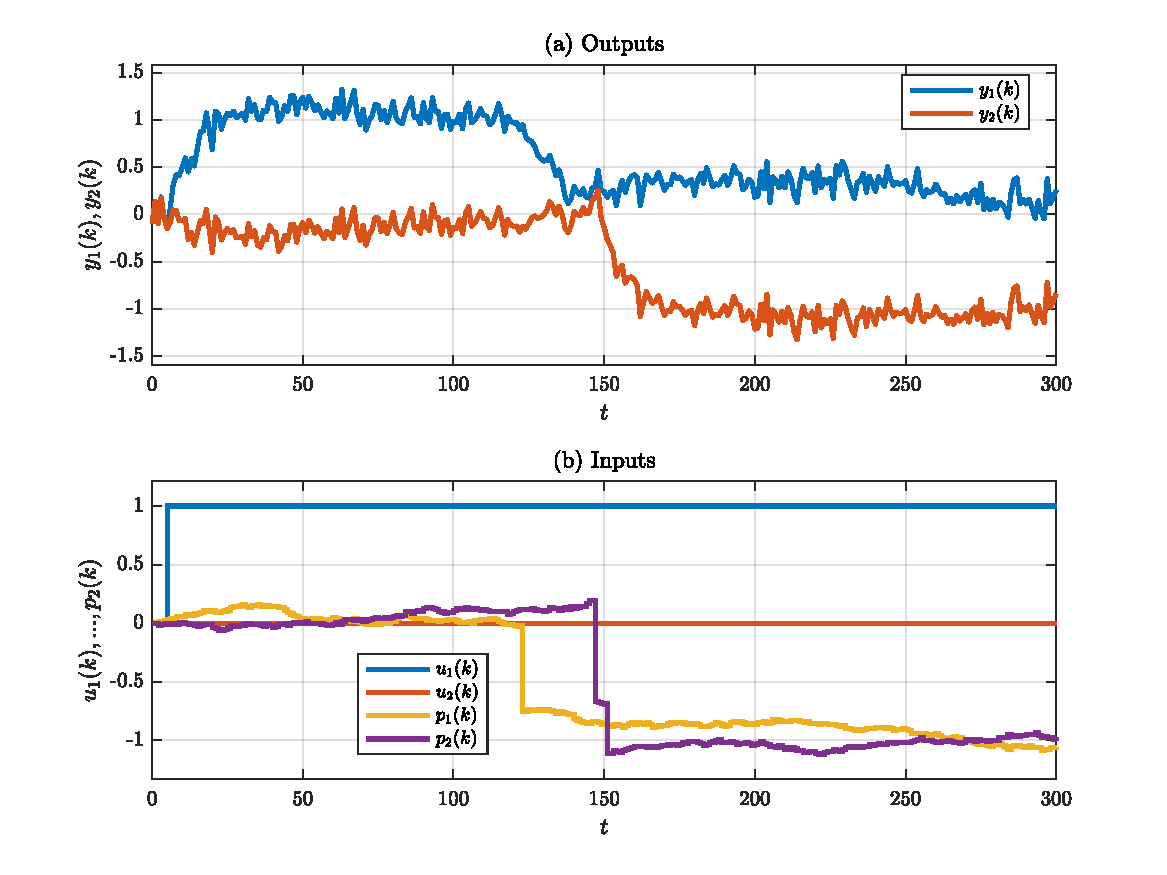
\includegraphics[width=15cm]{images/rod-obs-sim-2-4-ioplot.pdf}
	\caption{Simulation of MIMO linear system with two RODD input disturbances}
	\label{fig:rodd-obs-sim-2-4-ioplot}
\end{figure}

\section{Ore feed disturbance estimation}

Outline notes:
\begin{outline}
	\1 Unlike previous simulations, this is a non-linear model.
	\1 Describe simulations with grinding simulation model with changing ore properties and changes (same as IFAC paper).
	\1 Describe various data sets generated and their intended use (estimation, validation, statistical performance evaluation).
	\1 Data set used for model identificaiton in Figure: Input-output data – Figure \ref{fig:rod_obs_sim_1_ioplot_P2DcTd4}.
	\1 How process model was identified.
	\1 Augmented model with RODD input step disturbance.
	\1 Use best observer from previous section (sequence pruning).
	\1 Table showing observer paramters.
	\1 Figure: comparison of observer estimates – Figure \ref{fig:rod_obs_sim_1_est_P2DcTd4}.
	\1 Figure: Observer responses to disturbances – Figure \ref{fig:sim_resp_plot}.
	\1 Describe overall performance comparison using metrics in Table \ref{tb:results}.
	\1 Discuss pro's and con's of MMKF observer (steady-state errors vs error in transitions, etc.)
	\1 Discuss applications and potential benefits (e.g. process control, RTO).
	\1 Describe sensitivity analysis simulations.
	\1 Describe sensitivity results:
	\2 (1) to model error, compare Kalman filter and MMKF. Figures \ref{fig:rod_obs_sim_sens_model_KF2_MSE_y_est} and \ref{fig:rod_obs_sim_sens_model_MMKF_MSE_y_est}.
	\2 (2) MMKF sensitivity to RODD model parameters. Figure  \ref{fig:rod_obs_sim_sens_rod_MMKF_MSE_y_est}
\end{outline}

\begin{figure}[htp]
	\centering
	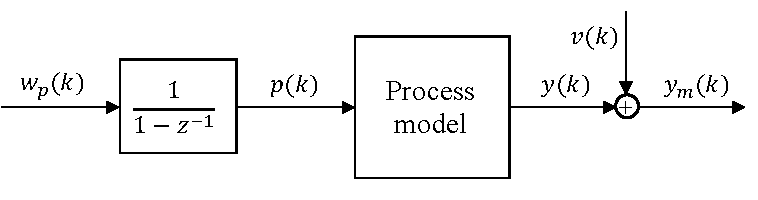
\includegraphics[width=10cm]{images/obs-model-diag.pdf}
	\caption{Observer model structure}
	\label{fig:obs_model}
\end{figure}

\begin{figure}[htp]
	\centering
	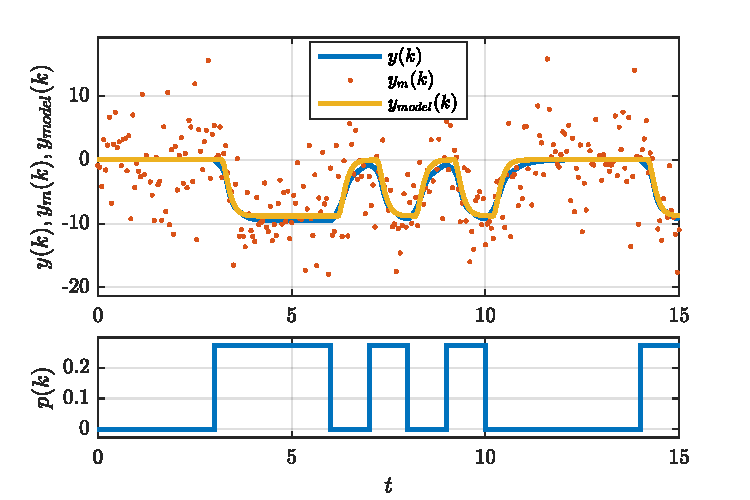
\includegraphics[width=12cm]{images/rod_obs_sim_1_ioplot_P2DcTd4.pdf}
	\caption{Observer model structure}
	\label{fig:rod_obs_sim_1_ioplot_P2DcTd4}
\end{figure}

\begin{figure}[htp]
	\centering
	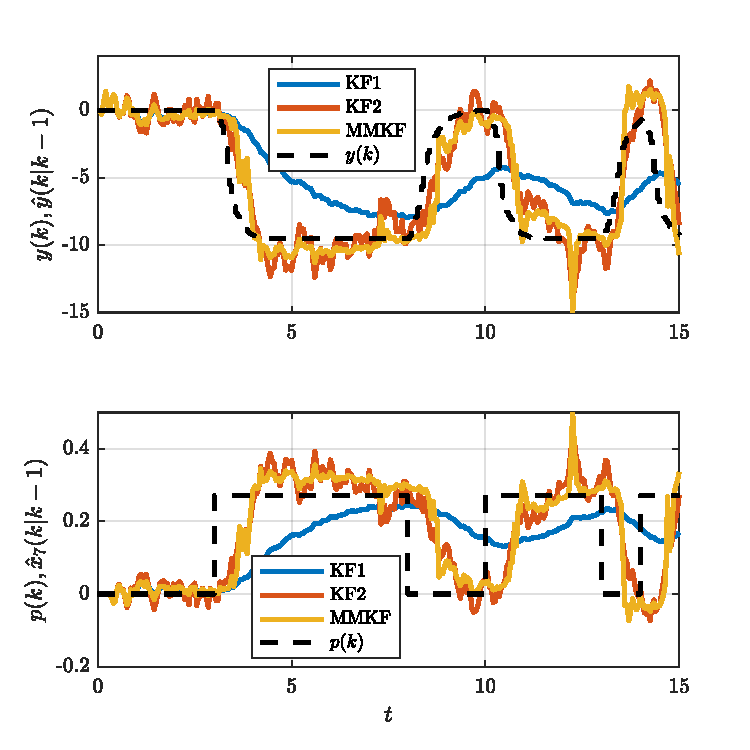
\includegraphics[width=12cm]{images/rod_obs_sim_1_est_P2DcTd4.pdf}
	\caption{Observer estimates}
	\label{fig:rod_obs_sim_1_est_P2DcTd4}
\end{figure}

\begin{figure}[htp]
	\centering
	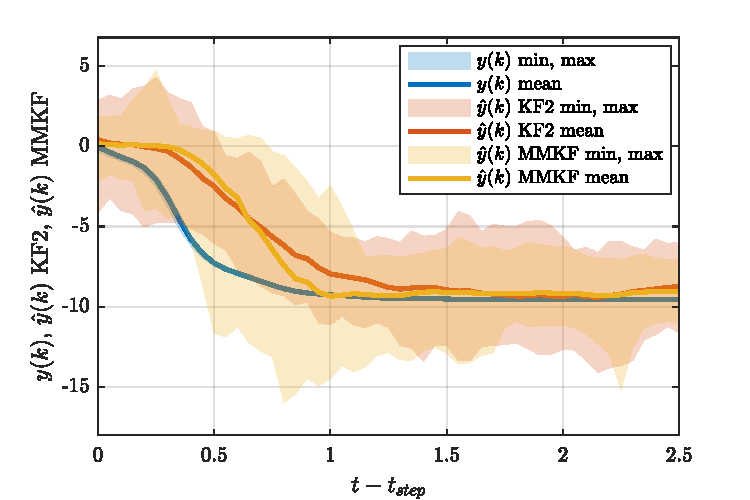
\includegraphics[width=12cm]{images/sim_resp_plot1_P2DcTd4.pdf}
	\caption{Average observer responses to step disturbances}
	\label{fig:sim_resp_plot}
\end{figure}

\begin{table}[hb]
	\begin{center}
		\caption{Observer performance metrics averaged over 50-days of simulation time.} \label{tb:results}
		% See: https://texblog.org/2019/06/03/control-the-width-of-table-columns-tabular-in-latex/
		\begin{tabular}{p{0.34\textwidth}>{\centering\arraybackslash}p{0.07\textwidth}>{\centering\arraybackslash}p{0.07\textwidth}>{\centering\arraybackslash}p{0.07\textwidth}>{\centering\arraybackslash}p{0.07\textwidth}>{\centering\arraybackslash}p{0.07\textwidth}}
			Metric & KF1 & KF2 & KF3 & MMKF & SKF \\
			\hline
			MSE($\hat{y}(k),y(k)$) overall          & 11.0 & 15.9 & 3.7 & 3.5 & 2.1 \\ 
			MSE($\hat{y}(k),y(k)$) transient       & 21.1 & 16.1 & 7.7 & 11.2 & 5.1 \\ 
			MSE($\hat{y}(k),y(k)$) steady-state & 7.9 & 15.9 & 2.5 & 1.1 & 1.1 \\ 
			Var($\hat{y}(k)$) steady-state          & 1.8 & 15.3 & 1.9 & 0.5 & 0.2 \\ 
			MSD($\hat{y}(k),y(k)$) steady-state       & 0.0 & 16.2 & 0.5 & 0.2 & 0.0 \\ 
			% Results for P2DcTd4
			%  Gc = -32.4 * exp(-0.2 * s) / (1 + 0.106*s)^2;
			%                                 KF1       KF3       AFMM        SKF  
			%  MSE                         11.118    3.7395     3.6991     2.0615
			%  MSE in transitions          20.687    7.7201      12.18     5.0674
			%  MSE in steady-state         8.1885     2.521     1.1028     1.1414
			%  Variance in steady-state    1.7723    1.9026    0.39281    0.23769
			%
			% Results for P2Dcd1_T
			%  Gc = -35.94 * exp(-0.05 * s) / ((1 + 0.235*s) * (1 + 0.161*s));
			%                                 KF1       KF3       AFMM        SKF  
			%  MSE                         10.707    3.7702     3.7283     1.9652
			%  MSE in transitions          21.052    7.7605     12.397     4.8145
			%  MSE in steady-state         7.5404    2.5486     1.0745      1.093
			%  Variance in steady-state    1.8111    1.9259    0.39282    0.24514
			
			% Updated results for P2DcTd4 with n_filt = 20, n_min = 18 after fixing
			% initialization between MC simulation runs.
			%  MSE                          11.01    3.6869     3.4952     1.8191
			%  MSE in transitions          21.137    7.7201     11.208     5.0722
			%  MSE in steady-state         7.9091    2.4523     1.1342     0.8232
			%  Variance in steady-state    1.8008    1.9026    0.47604    0.23759
			
			\hline
		\end{tabular}
	\end{center}
\end{table}

\begin{figure}[htp]
	\centering
	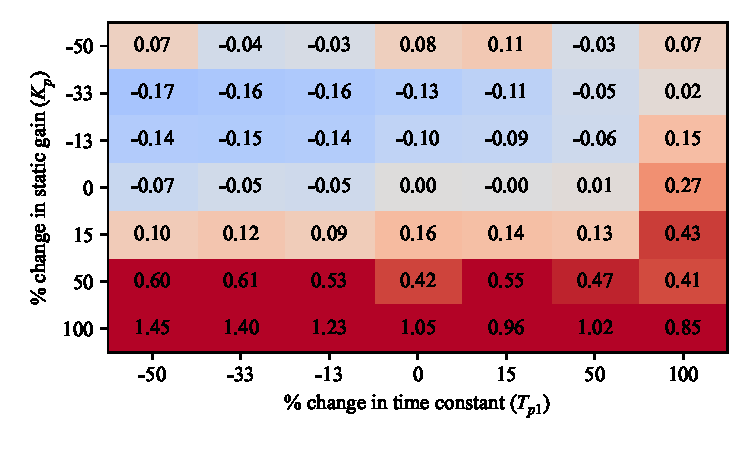
\includegraphics[width=12.5cm]{images/rod_obs_sim_sens_model_KF2_MSE_y_est.pdf}
	\caption{Sensitivity of KF2 estimates to changes in model parameters}
	\label{fig:rod_obs_sim_sens_model_KF2_MSE_y_est}
\end{figure}

\begin{figure}[htp]
	\centering
	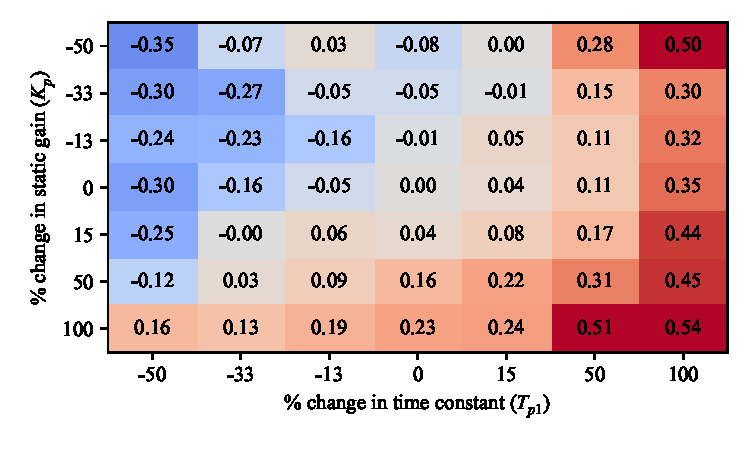
\includegraphics[width=12.5cm]{images/rod_obs_sim_sens_model_MMKF_MSE_y_est.pdf}
	\caption{Sensitivity of MMKF observer estimates to changes in model parameters}
	\label{fig:rod_obs_sim_sens_model_MMKF_MSE_y_est}
\end{figure}

\begin{figure}[htp]
	\centering
	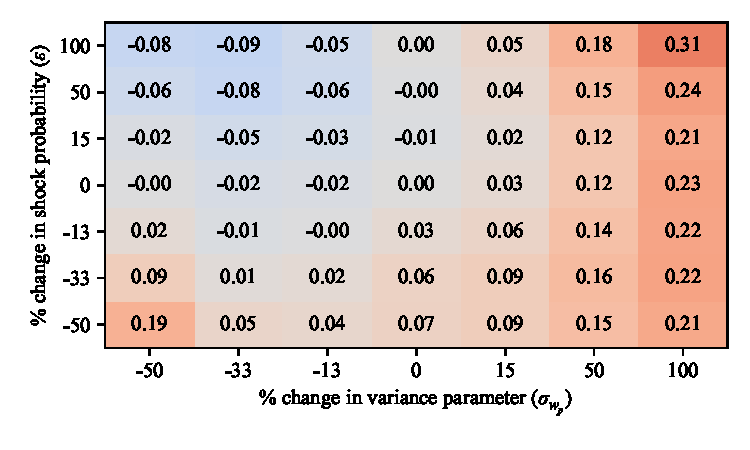
\includegraphics[width=12.5cm]{images/rod_obs_sim_sens_rod_MMKF_MSE_y_est.pdf}
	\caption{Sensitivity of MMKF observer estimates to changes in RODD parameters}
	\label{fig:rod_obs_sim_sens_rod_MMKF_MSE_y_est}
\end{figure}


\section{Grinding circuit control simulation}

Outline notes:
\begin{itemize}
	\item Grinding simulation model in closed loop with MPC controller.
	\item Diagram of feedback system – Figure \ref{fig:sim-mpc-diag}
	\item Table of results - Performance metrics — e.g. tracking error.
	\item Robustness?  E.g. stability margins.
\end{itemize}

\begin{figure}[htp]
	\centering
	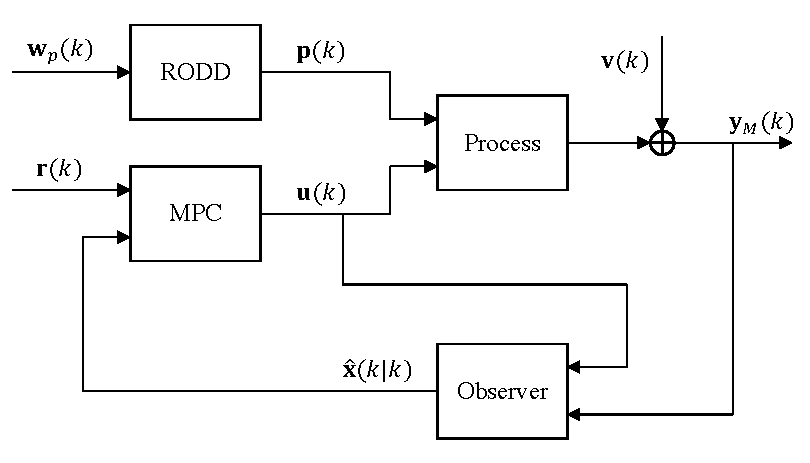
\includegraphics[width=12cm]{images/sim-mpc-diag.pdf}
	\caption{Functional diagram of the simulated feedback control system}
	\label{fig:sim-mpc-diag}
\end{figure}